%%% Time-stamp: <mainrep.tex 19:57, 17 Jul 2016 by P Sunthar>
%%% $Log:$
% This document describes how to use iitbreport style
%********************************************************************

%\documentclass[11pt,a4paper,openright]{report}
\documentclass[twoside]{iitbreport}

%% Default spacing: 1.5
%% Default font size: 12pt
%% Default font: txfonts (similar to times new roman)

%% Selectively comment out sections that you want to be left out but
%% maintaining the page numbers and other \ref
\includeonly{%
  intro/introduction,
  dem/dem_intro,
  lit/literature,
  expt/experimental,
  rnd/results,
  dec,abs,pub,ack
}

%%% Some commonly used packages (make sure your LaTeX installation
%%% contains these packages, if not ask your senior to help installing
%%% the packages)

\usepackage{booktabs}
\graphicspath{{expt/}}

\usepackage{physics}
\usepackage{subcaption}
\usepackage{tikz}

%%% Macro definitions for Commonly used symbols
\newcommand{\Rey}{\ensuremath{\mathrm{Re}}}
\newcommand{\avg}[1]{\ensuremath{\overline{#1}}}
\newcommand{\tenpow}[1]{\ensuremath{\times 10^{#1}}}
\newcommand{\pder}[2]{\ensuremath{\frac{\partial#1}{\partial#2}}}

% Referencing macros
\newcommand{\Eqref}[1]{Equation~\eqref{#1}}
\newcommand{\Tabref}[1]{Table~\ref{#1}}
\newcommand{\Figref}[1]{Figure~\ref{#1}}
\newcommand{\Appref}[1]{Appendix~\ref{#1}}


\begin{document}

%%********************************Frontmatter***********************
% In frontmatter everything comes with roman numbering
\pagenumbering{roman}
\setcounter{page}{1}

%*******************************************************************
%                         Title Page
%*******************************************************************
\title{Essential \LaTeX\ Templates for Report Writing}
\author{My name}

%% Print the date. Today's date comes by default, change it here to
%% other date format, if required:

%\date{\today}
%\date{10 Mar 2016}


%% The type of the report can be set here

\reporttype{A Seminar Report}
%\reporttype{A Thesis}
%\reporttype{A Dissertation}
%\reporttype{A Project Report}

%% Name of the degree
\degree{Doctor of Philosophy}
%\degree{Master of Technology}


%% Department/Centre Name
\dept{Department of Chemical Engineering}

%% Supervisor and cosupervisor/excosupervisor are not essential parts
%% of a report title page, as it is your report!

%% But if you **have** to put it uncomment these
%\supervisor{Supervisor name}
%\cosupervisor{Co-super name}
%\excosupervisor{External Supervisor}

%% Roll number
\rollnum{Roll No. ....}

\maketitle

%*******************************************************************
%                         Copyright Page
%*******************************************************************
%\mycopyright

%*******************************************************************
%                         Dedication Page
%*******************************************************************
\dedication[Dedicated to \ldots]
%\addintoc{Dedication}

%*******************************************************************
%                        Certificate Page
%*******************************************************************
%\makecertificate[change title name]{report type}
\makecertificate{seminar report}
%\makecertificate{thesis}
%\makecertificate{dissertation}
%\makecertificate{project report}

%\addintoc{Certificate}

%*******************************************************************
%                         Approval Sheet
%*******************************************************************
%\makeapproval{thesis}
%\makeapproval{dissertation}

%*******************************************************************
%                          Declaration
%*******************************************************************
%==================================dec.tex================================
%
\begin{Declaration}
\noindent
I declare that this written submission represents my ideas in my own words and where others' ideas or words have been included, I have adequately cited and referenced the original sources. I declare that I have properly and accurately acknowledged all sources used in the production of this report. I also declare that I have adhered to all principles of academic honesty and integrity and have not misrepresented or fabricated or falsified any idea/data/fact/source in my submission. I understand that any violation of the above will be a cause for disciplinary action by the Institute and can also evoke penal action from the sources which have thus not been properly cited or from whom proper permission has not been taken when needed.

%
%
%
%
%
%
%

\DecSign[\today]



%
\end{Declaration}
%========================================================================

















%\addintoc{Declaration}

%******************************************************************
%                          Abstract
%******************************************************************
%============================= abs.tex================================
\begin{Abstract}
This document contains essential templates required to write technical
reports using \LaTeX.  Particularly it shows how to create an
equation, figure, table, symbols list, and bibliographic citation in a \LaTeX\
document.
%
%
%
%
%
\end{Abstract}
%=======================================================================



%******************************************************************
%                         Contents list
%******************************************************************
%\figurespagefalse
%\tablespagefalse
\makecontents % Creats toc, lof, and lot

%******************************************************************
%                        Notations
%******************************************************************
\notations[4cm]{List of Symbols}

%%********************************Mainmatter***********************
% In mainmatter everything comes with arabic numbering
\cleardoublepage
\setcounter{page}{1}
\pagenumbering{arabic}

%******************************************************************
%                         Chapters
%******************************************************************

\newcommand{\etas}{\ensuremath{\eta_{\mathrm{s}}}}


\chapter{Introduction}


This document contains commonly used essential templates to write a
\LaTeX\ document. This document is to be used along with the files and
folders provided. Writing a \LaTeX\ document is very simple.  Often
students need only very simple constructs.  This document shows
certain essential features that almost all technical report writing
requires. Please consult the PDF file for the output of the document,
and then look at the corresponding \LaTeX\ file to reproduce it.  The
document illustrates the following constructs
\begin{itemize}
\item Unnumbered and numbered Lists
\item Equations
\item Defining short macros for frequently used symbols
\item Bibliography
\item Figures
\item Tables
\end{itemize}

The normal procedure for compiling a \LaTeX\ document that contains
bibliographic entries is to follow the following steps
\begin{enumerate}
\item \verb|pdflatex mainrep|
\item \verb|bibtex mainrep|
\item \verb|pdflatex mainrep|
\item \verb|pdflatex mainrep|
\end{enumerate}
In the above example \verb|mainrep| is the main \LaTeX\ file.


\section{First section of this chapter}

This is the first chapter, which resides in a directory (folder)
intro. Each chapter can contain \verb|section|, \verb|subsection|
and so on.

\subsection{Equations and Math symbols}


Equations should be set in a separate mode.  For details on getting
various types of aligned equations, consult the \AmS-\LaTeX\
documentation \verb|amsldoc.pdf|. Simple equations are set as
\begin{equation}
\label{eq:sinx}
\int \mathrm{d}x \; \cos x =  \sin x
\end{equation}
Equation~\eqref{eq:sinx} is the integral of the cosine
function. Mathematical symbols must always be put inside \verb|$$|,
when they appear outside a math environment (such as \verb|equation|,
\verb|align|, \verb|gather|, etc).  The symbol ``ex'' must be written as
$x$ and not as x.  

Another commonly used construct for equations is the \verb|align|
environment to align several equations along a vertical line. It is
usually the $=$ sign across which the alignment is done.  The
point of alignment for each equation is specified using the ampersand symbol 
\begin{align}
a &= b  \\
a + e + f + g & = m + n + z \\
x + 2 & = x^{3} + 3 x^{2} + 2 x + 5
\end{align}

\subsection{Commonly used Symbols}
For mathematical symbols it is very convenient to define frequently
used symbols as a short macro. For example if you are to be using the
symbol $\eta_{\mathrm{s}}$ frequently it is convenient to define it in
as:\\
\verb|\newcommand{\etas}{\ensuremath{\eta_{\mathrm{s}}}}| \\
in the preamble and to simply refer it to in the text as \etas\ or in
a mathematical equation as $\etas = \eta \, ( 1 + \phi)$.
%%
%

\section{How to write nomenclature} 

\subsection{General guidelines:}
\begin{enumerate}	
	\item Use \verb|\nomenclature[prefix]{symbol}{description}| for symbols, the best place for this command is immediately after you introduce the symbol for the first time
	\item Shorten the long command:\\ \verb|\newcommand{\nm}[2]{\nomenclature{#1}{#2}}|
	\item Create compiler for nomenclature with the given code: \\
	\textbf{makeindex \%.nlo -s nomencl.ist -o \%.nls -t \%.nlg }\\
	For TeXstudio: go to options > build > user command > write- `user1: Nomenclature' amd paste the above code\\
	For compiling the nomenclature: go to tools > user > Nomenclature	
\end{enumerate}	

\subsection{Grouped nomenclature}
\begin{enumerate}
\item For acronyms, use:\\
 \verb|\nmA[sorting letter]{symbol}{descritpon}|
\item For roman symbols, use:\\
\verb|\nmR[sorting letter]{symbol}{descritpon}|
\item For greek symbols, use:\\
 \verb|\nmG[sorting letter]{symbol}{descritpon}|
 \item For superscripts, use:\\
 \verb|\nmS[sorting letter]{symbol}{descritpon}|
 \item For subscripts, use:\\
 \verb|\nms[sorting letter]{symbol}{descritpon}| 
 \item For any other symbol, use:\\
 \verb|\nmX[sorting letter]{symbol}{descritpon}|\\
 Name of other symbols can be changed with \verb|\OtherSym{Name of symbols}|
\end{enumerate}
%%
\subsection{Some examples}
\begin{enumerate}
\item \verb|\nmA[FF]{FFA}{Free fatty acid}|
\item \verb|\nmA[AO]{AOR}{Angle of repose}|
\item \verb|\nmR[Ra]{$R$}{Radius of circle}|
\item \verb|\nmR[ra]{$r$}{Intrinsic length}|
\item \verb|\nmR[Gr]{$G_\mathrm{r}$}{Gravity}|
\item \verb|\nmG[al]{$\alpha_{\mathrm{a}}$}{Angular acceleration}|
\item \verb|\nmG[et]{$\eta$}{Viscosity}|
\item \verb|\nmG[be]{$\beta$}{Shape factor}|
\item \verb|\nmS[v]{$v$}{Vapor phase}|
\item \verb|\nmS[g]{$g$}{Gas phase}|
\item \verb|\nms[i]{$i$}{Indices}|
\item \verb|\nms[x]{$x$}{Variable in x-direction}|
\item \verb|\nmX[f]{foo}{foo|
\end{enumerate} 

\nmA[FF]{FFA}{Free fatty acid}
\nmA[AO]{AOR}{Angle of repose}


\nmR[Ra]{$R$}{Radius of circle}
\nmR[ra]{$r$}{Intrinsic length}
%\nmR[Gr]{$G_\mathrm{r}$}{Gravity}


\nmG[al]{$\alpha_{\mathrm{a}}$}{Angular acceleration}
\nmG[et]{$\eta$}{Viscosity}
%\nmG[be]{$\beta$}{Shape factor}


\nmS[v]{$v$}{Vapor phase}
\nmS[g]{$g$}{Gas phase}


\nms[i]{$i$}{Indices}
\nms[x]{$x$}{Variable in x-direction}


\nmX[f]{foo}{foo}


%%


%%% Local Variables: 
%%% mode: latex
%%% TeX-master: "../mainrep"
%%% End: 

\chapter{Discrete element method}

Discrete element method (DEM) is a numerical tool used to model discrete systems by
solving Newton's equations of motion on each particle in the system. It also
allows to model continuous systems by discretizing into particles.


\section{Introduction}
\label{sec:introduction}

Let's first discuss a real life example before discussing the algorithm of
DEM.\@ Consider sand, sand consists of many discrete particles which has mass, a
definite shape and other properties. We want to know the dynamics of sand
flowing through various bodies such as a hopper, hour-glass or a filter. One way
of modelling such system is to assume the sand to be a continuum and by
conservation laws we can solve for various macroscopic properties such as
stress, strain etc, just like solving for a fluid or solid.

Unfortunately, a system like sand, behaves differently at different places. As
an example consider the behaviour of sand flowing under gravity in an hourglass
(see fig \ref{fig:hourglass}) \footnote{taken from
  \href{https://www.istockphoto.com/in/videos/hourglass?sort=mostpopular&offlinecontent=include&phrase=hourglass}
  {istockphoto}.}  and second example of particles getting jammed in a hopper
(see fig \ref{fig:hopper_jam} \footnote{taken from
  \href{http://webhome.phy.duke.edu/~jt41/research.html}{Junyao Tang's Home
    Page}}). We can observe in hourglass example as the sand flows like fluid
while it passes through the opening. By seeing this part and considering to
model the system as continuum would be would be a choice. But as soon as as it
hits the ground, rather than behaving like a fluid and flowing towards the wall,
it forms into a mountain. In the second example it is even more ambiguous,
rather than flowing out completely particles gets jammed.


\begin{figure}[h]
  \begin{subfigure}{0.5\textwidth}
    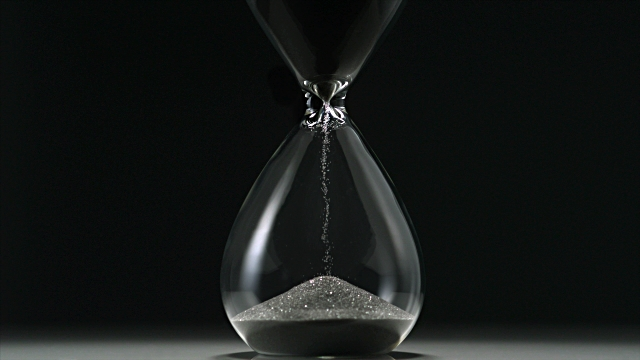
\includegraphics[width=0.9\linewidth, height=5cm]{dem/doc_images/hourglass}
    \caption{Sand exhibiting different behaviour in an hourglass (Reproduced from \href{https://www.istockphoto.com/in/videos/hourglass?sort=mostpopular&offlinecontent=include&phrase=hourglass}{istockphoto})}
    \label{fig:hourglass}
  \end{subfigure}
  \begin{subfigure}{0.5\textwidth}
    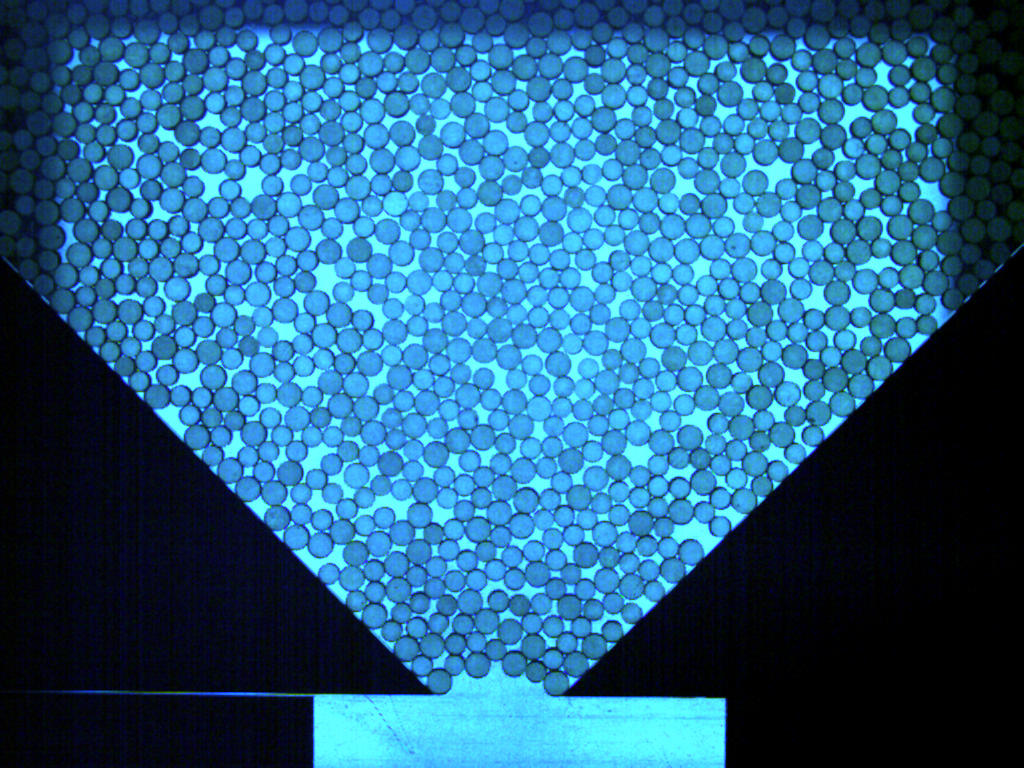
\includegraphics[width=0.9\linewidth, height=5cm]{dem/doc_images/hopper_jam}
    \caption{Particles jammed in a hopper. (Reproduced from
      \href{http://webhome.phy.duke.edu/~jt41/research.html}{Junyao Tang's Home
    Page})}
    \label{fig:hopper_jam}
  \end{subfigure}

  \caption{Unexpected behaviour of a system with discrete particles}
  \label{fig:dem_introduction}
\end{figure}

In 1979 \citeauthor{Cundall_1979} introduced DEM to model such system. They
models the system using many discrete particles having specific shape, mass,
material properties and which interact at surfaces, and their dynamics is
captures using Newton's law of motion.

In the present chapter we will discuss in detail of DEM implementation. In the
next section the steps involved to set up a DEM simulation is discussed. In the
later section contact force models are discussed. After that the simulation
parameters, such as spring stiffness, damping coefficient and other parameters
which govern the simulation are discussed.


\section{Discrete Element Method}

It is a numerical method introduced by \cite{Cundall_1979},
used to model the behavior of large number of particles having finite
mass and radius which interact at their surfaces. The governing
equation of motion for such a particle can be written using Newton's
laws.

\begin{align}
  \label{eq:newton_equation_of_motion}
  \frac{d^2 \vec{x}}{dt^2} = \vec{F}(\vec{x}, \vec{v}, m)\\
  \frac{d^2 \vec{\omega}}{dt^2} = \vec{M}(\vec{x}, \vec{v}, m)
\end{align}

Where $\vec{F}$, $\vec{M}$ is the force and moment acting on the
particle. m, $\vec{v}$, $\vec{x}$ are the mass, position and velocity
of the particle.
The force $\vec{F}$ in equation\ref{eq:newton_equation_of_motion} is
the one to be computed during each time step. This force arises due to
collision of particles.

% \begin{figure}
%   \centering
%   \includegraphics[scale=0.5]{dem/two_pars_in_contact}
%   \caption{Two spherical particles in contact}
%   \label{fig:tspc}
% \end{figure}

Before studying the interaction of a particle with wall or any other
spherical particle, lets consider a spherical particle with mass m
freely falling under gravity. For such a model, the governing
differential equation can be written as

\begin{align}
  \label{eq:free_fall}
  \frac{d^2 \vec{x}}{dt^2} = \vec{g}\\
  \frac{d^2 \vec{\omega}}{dt^2} = 0
\end{align}

Such a differential equation \eqref{eq:free_fall} governs a scene like
in figure \eqref{fig:free_fall}

\begin{figure}[htb]
  \centering

  \begin{subfigure}{.5\textwidth}
    \centering
    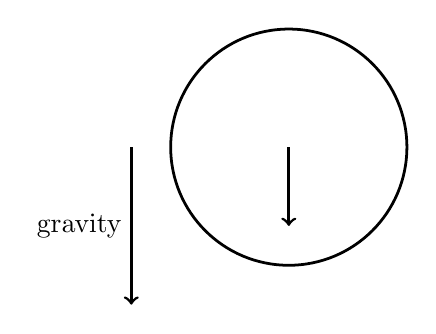
\begin{tikzpicture}
      % ---------------------------------------------
      \draw[line width=1pt] (0, 0) circle[radius=1.5];
      \draw[->,line width=1pt] (0, 0) -- (0, -1);
      \draw[->,line width=1pt] (-2, 0) -- (-2, -2);
      \node[left] at (-2, -1) {$\text{gravity}$};
    \end{tikzpicture}
    \caption{A freely falling Sphere}
    \label{fig:free_fall}
  \end{subfigure}%

  \begin{subfigure}{.5\textwidth}
    \centering
    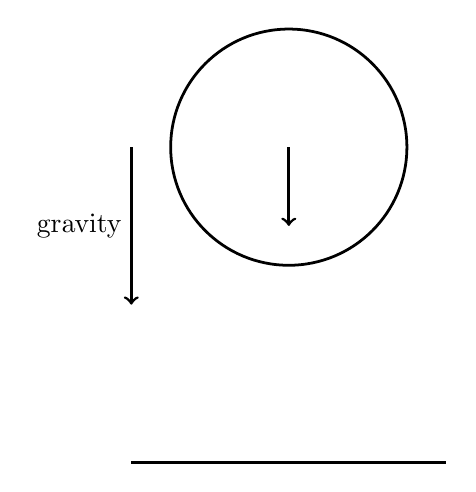
\begin{tikzpicture}
      \draw[line width=1pt] (0, 0) circle[radius=1.5];
      \draw[->,line width=1pt] (0, 0) -- (0, -1);
      \draw[->,line width=1pt] (-2, 0) -- (-2, -2);
      \draw[line width=1pt] (-2, -4) -- (2, -4);
      \node[left] at (-2, -1) {$\text{gravity}$};
    \end{tikzpicture}
    \caption{A freely falling Sphere onto a wall}
    \label{fig:bounce_back}
  \end{subfigure}

  \caption{Behaviour of sphere under different conditions}
  \label{fig:sphere_intro}
\end{figure}

In freely falling situation, the particle doesn't see any obstacles,
and follows a straight line path.

Now assume that there is a wall obstructing the motion of this
spherical ball.  As the ball hits the wall it has to bounce back
\eqref{fig:bounce_back}, because of the repulsion force from the
wall. There are two ways to model such a behavior.

\begin{itemize}
\item Event driven method (hard particles)
\item Discrete element methods (soft particles)
\end{itemize}


Present work deals with Discrete element method, with a little introduction
to Event driven method.

\section{Discrete element method (DEM)}
\label{sec:edm}

In this method at every instant of time the ball is checked if it is
in contact with any other particle or wall. If it is, then the force
is computed from the relative positions of the overlapping
particles. By using such force($\vec{F}$) \eqref{eq:newton_equation_of_motion} is
integrated using Euler or ARK2.

\subsection{Force calculation}
\label{sec:force}

\begin{figure}[htb]
  \centering
  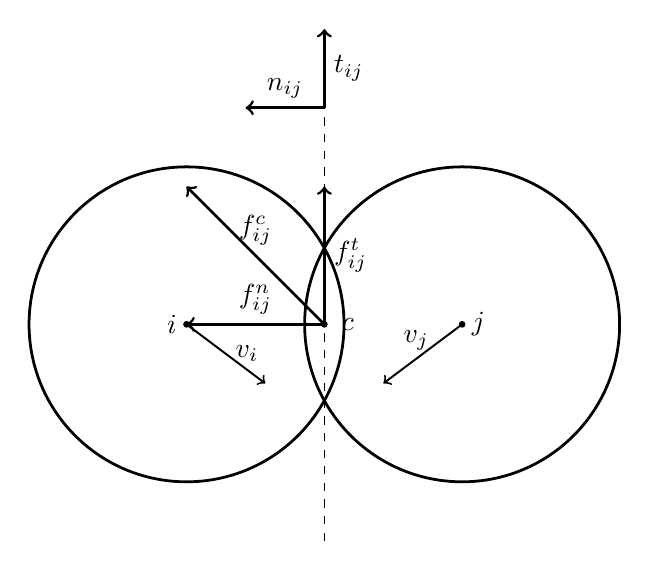
\begin{tikzpicture}
    % ---------------------------------------------
    \draw[line width=1pt] (0, 0) circle[radius=2];
    \draw[fill] (0,0) circle[radius=1pt];
    \node[left] at (0, 0) {$i$};
    \draw[line width=1pt] (3.5, 0) circle[radius=2];
    \draw[fill] (3.5, 0) circle[radius=1pt];
    \node[right] at (3.5, 0) {$j$};

    % draw normal vector
    \draw[dashed] (1.75, -2.75) -- (1.75, 3.75);
    \draw[->, line width=1pt] (1.75, 2.75) -- (0.75, 2.75);
    \node[above] at (1.25, 2.75) {$n_{ij}$};
    \draw[->, line width=1pt] (1.75, 2.75) -- (1.75, 3.75);
    \node[right] at (1.75, 3.25) {$t_{ij}$};

    % draw force components
    \draw[->, line width=1pt] (1.75, 0) -- (0.0, 1.75);
    \node[above] at (0.875, 0.875) {$f^c_{ij}$};
    \draw[->, line width=1pt] (1.75, 0) -- (0.0, 0);
    \node[above] at (0.875, 0) {$f^n_{ij}$};
    \draw[->, line width=1pt] (1.75, 0) -- (1.75, 1.75);
    \node[right] at (1.75, 0.875) {$f^t_{ij}$};

    % contact point
    \draw[fill] (1.75, 0) circle[radius=1pt];
    \node[right] at (1.85, 0) {$c$};

    % velocities
    \draw[->, line width=0.7pt] (0, 0) -- (1., -.75);
    \node[right] at (0.5, -0.375) {$v_i$};
    \draw[->, line width=0.7pt] (3.5, 0) -- (2.5, -.75);
    \node[left] at (3.2, -0.20) {$v_j$};

  \end{tikzpicture}
  \caption{Two spherical particles in contact}
  \label{fig:tspc}
\end{figure}

\begin{equation}
  \label{eq:overlap}
  \delta = (r_i + r_j) - |\vec{X}_{i} - \vec{X}_{j}|
\end{equation}

Say two particles \eqref{fig:tspc} i and j with radii $r_{i}$ and
$r_{j}$, are in contact if $\delta$ \eqref{eq:overlap} is positive.
The particle i has linear velocity $\vec{V}_{i}$ and angular velocity
of $\vec{\omega}_{i}$ particle j has linear velocity $\vec{V}_{j}$ angular
velocity of $\vec{\omega}_{j}$.

The unit normal vector along particle i to particle j  is given by

\begin{equation}
  \label{eq:normal_unit}
  \vec{n}_{ij} = \frac{\vec{X}_{j} - \vec{X}_{i}}{|\vec{X}_{j} - \vec{X}_{i}|}
\end{equation}

The relative velocity of point of contact becomes

\begin{equation}
  \label{eq:relative}
  \vec{V}_{ij} = \vec{V}_{i} - \vec{V}_{j} +
  (r_{i} \vec{\omega}_{i} + r_{j} \vec{\omega}_{j}) \times \vec{n}_{ij}
\end{equation}

Therefore the normal and tangential components of contact velocity are

\begin{equation}
  \label{eq:normal_vel}
  \vec{V}_{nij} = \vec{V}_{ij} \cdot \vec{n}_{ij} \vec{n}_{ij}
\end{equation}

\begin{equation}
  \label{eq:tang_vel}
  \vec{V}_{tij} = \vec{V}_{ij} - \vec{V}_{ij} \cdot \vec{n}_{ij} \vec{n}_{ij}
\end{equation}

The tangent to the plane of contact is

\begin{equation}
  \label{eq:tang_unit}
  \vec{t}_{ij} = \frac{\vec{V}_{tij}}{|\vec{V}_{tij}|}
\end{equation}


Discrete element method is a soft sphere approach. In soft sphere
approach the overlap between two particles is described by a spring
and a dashpot in both normal and tangential direction. Generally, when
two particles collide, there will be a repulsion force on both the
particles. This repulsive force is represented by springs, whose
magnitude depends on the overlap amount. Similarly, when a collision
occurs, there will be damping of energy due to deformation of the body
and the friction force between the particles. This damping is taken
care by the dashpot between the particles. The respective spring and
damping coefficients depend on the coefficient of restitution between
the colliding particles and the material properties of the colliding
particles.


The normal ($\vec{F}_{nij}$) and tangential ($\vec{F}_{tij}$)
components of the contact force ($\vec{F}_{ij}$) at time t can be
written as

\begin{equation}
  \label{eq:normal_force}
  \vec{F}_{nij} =  \vec{F}_{nij}^S +  \vec{F}_{nij}^D
\end{equation}

\begin{equation}
  \label{eq:tangential_force}
  \vec{F}_{tij} =  \vec{F}_{tij}^S +  \vec{F}_{tij}^D
\end{equation}

In a linear force, normal spring force $\vec{F}_{nij}$ is computed from the overlap
amount between the particles. This force is always repulsive in nature
and it conserves the energy of the colliding particles.

\begin{equation}
  \label{eq:normal_spring_force}
  \vec{F}_{nij}^S = -k_n \> \delta_n \> \vec{n}_{ij}
\end{equation}

Since as discussed, when two particle collide there will be loss in
energy due to friction, body deformation, rolling friction and many
more. To model such energy loss, we consider a single damping force,
which depends on the coefficient of restitution between particles, and
the force opposes the velocity. Such damping force can be written as

\begin{equation}
  \label{eq:normal_damping_force}
  \vec{F}_{nij}^D = -\eta_n  (\vec{V}_{ij} \cdot \vec{n}_{ij}) \> \vec{n}_{ij}
\end{equation}


Tangential spring force is calculated in a different way. At the
instantiation of the a spring is attached in tangential direction, and
as time proceeds, the elongation of the spring is noted. At every time
step depending on the displacement of the spring the force is
computed.

\begin{equation}
  \label{eq:tang_spring_force}
  \vec{F}_{tij}^S = -k_t \> \vec{\delta_t}
\end{equation}

Where $ \vec{\delta_t} $ at the instantiation of the contact
can be written as

\begin{equation}
  \label{eq:tang_disp}
 \vec{\delta_t} = \vec{V}_{tij} \> \Delta t
\end{equation}

And after time $\Delta t$

\begin{equation}
  \label{eq:tang_disp}
 \vec{\delta}_{t + \Delta t} = \vec{\delta}_{t} + \vec{V}_{tij} \> \Delta t
\end{equation}

Where as tangential damping force is similar to normal damping force, which can be
written as

\begin{equation}
  \label{eq:tang_damp_force}
  \vec{F}_{tij}^D = -\eta_t \> \vec{V}_{tij}
\end{equation}

With such a tangential law, the force opposing the motion will increase indefinitely,
to make it finite, Coloumb condition is applied. It is given as follows

\begin{equation}
  \label{eq:coloumb}
  |\vec{F}_{tij}| > \mu \> |\vec{F}_{nij}|
\end{equation}

where $\mu$ is coefficient of friction.

\subsection{Computing normal and tangential coefficients}

We defined the force laws between two colliding spheres, these forces are
dependent on the spring and dashpot coefficients. These are computed as follows,
Generally while defining collision, material properties and coefficient of restitution is
specified, using these values, we need to come up with the coefficients.

In linear force model from MFIX DEM we have normal coefficient of restitution as
\begin{equation}
  \label{eq:damping_coefficient}
  \eta_{n} = \frac{2 \> \sqrt{m_{eff}k_{n}}|\ln e_n|}{\sqrt{\pi^2 + \ln^2e_{n}}}
\end{equation}


\section{Particle Wall collision}
\label{sec:PWColl}

Till now particle  collision is modelled. Particle wall
collision can be modelled in the following way. A point and normal to
the wall is need to be defined \ref{fig:wall_description}

\begin{figure}
  \centering
  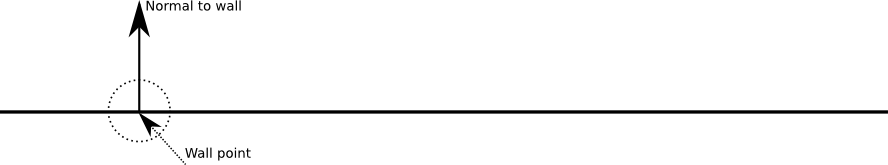
\includegraphics[scale=2.]{dem/doc_images/wall_description}
  \caption{Describing a wall in DEM Simulation}
  \label{fig:wall_description}
\end{figure}


After defining a wall, to check if a given particle of radius r in
contact with the Paine the following condition is to be satisfied.

Say that $\vec{n}_w$ is the normal for wall, and the vector joining
the wall point and the particle is $\vec{r}_{wi}$. The perpendicular
distance between wall and the particle can be computed using

\begin{align}
  \label{eq:perpendicular_dist}
    Perpendicular Distance(PR) =  \vec{r}_{wi} \cdot  \vec{n}_w
\end{align}

If $r - PR $ is positive, then the particle is overlapping the wall,
such $r - PR$ is the overlap amount. Where $r$ is the radius of the
particle\ref{fig:particle_wall_collision}. From such overlap amount
and material properties force on the particle can be computed using
\eqref{eq:normal_force} and \eqref{eq:tangential_force}

\begin{figure}
  \centering
  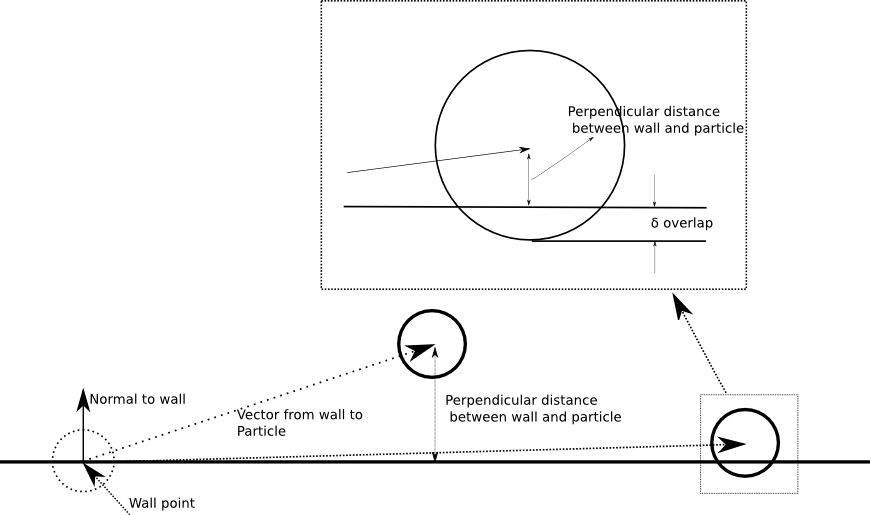
\includegraphics[scale=1.5]{dem/doc_images/particle_wall_collision.png}
  \caption{Particle and wall colliding}
  \label{fig:particle_wall_collision}
\end{figure}



\subsection{Tangential force}
\label{sec:tangential-force}

Tangential force is divided into two phases, one is sticking and the other one
is sliding. Sticking is when the tangential force between two particles is less
than the Coulomb friction, in this condition particles at contact point won't
move, rather the centers of the particles will move elastically. In sliding
motion, the tangential force exceeds the friction force and the particles starts
to slide. In sliding condition the tangential force is bounded by Coulomb
frictional force.

Similar to normal component tangential component is also composed
of a conservative and non conservative part. Unlike conservative normal contact
force, conservative part in tangential direction is complicated. At a given time
step, in normal force law one computes the overlap amount at that instant and
uses it for force, but in tangential direction one needs to keep track of the
spheres which are in overlap and increment those springs elongation. The force
law is given by

\begin{equation}
  \label{eq:tangential_force_spring_damping}
  \vec{f}_{t0} = -k_t \, \vec{\delta}_t - \gamma_t \, \vec{v}_t
\end{equation}


\begin{equation*}
  \vec{\delta}_t = \vec{\delta}_t + \vec{v}_t \, dt
\end{equation*}

As we can observe from equation \ref{eq:tangential_force_spring_damping},
the conservative part is in the opposite direction of the elongation similar
to the normal conservative part. The non conservative part is in the opposite
direction of the tangential velocity which will reduce the energy of the
particle.

Once we compute the tangential force from the springs elongation, we compare it
with maximum allowed tangential force, i.e., static friction $\mu_s \, f_n$ if
the tangential force exceeds static friction then the particles start to slide
the tangential force is adjusted to sliding friction.

\begin{equation}
  \label{eq:tangential_force_spring_damping}
  f_t = \max(\norm{f_{t0}}, \mu_s f_n) \vec{t}
\end{equation}
where $\vec{t}$ is the direction of $\frac{\vec{f}_{t0}}{\norm{\vec{f}_{t0}}}$.



\section{Application to Rigid body simulation}
\label{sec:appl-rigid-body}

DEM can be applied to rigid body simulation to evaluate the forces between rigid
bodies in collision. The modelling process starts by discretizing the rigid
bodies into particles (Fig~\ref{fig:rigid_body_particles} \footnote{Taken from Nvidia}).


\begin{figure}
  \centering
  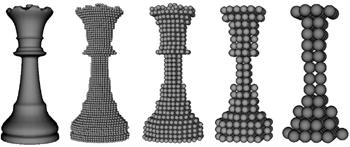
\includegraphics[width=0.9\linewidth, height=5cm]{dem/doc_images/grid_to_particles}
  \caption{Rigid body discretized as particles. (Reproduced from
    \href{https://developer.nvidia.com/gpugems/GPUGems3/gpugems3_ch29.html}{nvidia})}
  \label{fig:rigid_body_particles}
\end{figure}


The dynamics of rigid body are simulated using Newton's equations. Consider a
body ($I$) having discretized into $k$ particles. Let the moment of inertia of
such body at a given time step be $I_I$. In a simulation loop at every time step
forces on the particle are evaluated using SPH and DEM due to interaction with
other particles of fluid and solid phases and are saved in $\dv{\vec{v}_k}{t}$.
After evaluating forces on particles, these forces are transferred to the center
of mass of the rigid body as a resulting moment and force.

\begin{eqnarray}
  \label{eq:rigid_body_newton_equation}
  M_I \dv{\vec{V}_I}{t} &=& \sum_{k \in I} m_k \dv{\vec{v}_k}{t}\\
  I_I \dv{\vec{\Omega}_I}{t} &=& \sum_{k \in I} m_k (\vec{r}_k - \vec{R}_I) \cross \dv{\vec{v}_k}{t}
\end{eqnarray}
After evaluating the resultant moment at the center of mass of the body, the
moment of inertia is computed through which angular velocity at the next time
step is evaluated. Using the angular velocity at the center, the linear
velocities of the particles are evaluated and used to propagate the particle
positions to next time.


Drawbacks of such algorithm is to evaluate the moment of inertia at each and
every time step, which is costly. To overcome such operation one can use
rotation matrices. Detailed explanation can be found at
\href{https://www.cs.cmu.edu/~baraff/sigcourse/notesd1.pdf}{Baraff unconstrained
  dynamics}.

\section{Bonded Discrete element method}
\label{sec:bond-discr-elem}

\citeauthor*{Potyondy_2004} in extended DEM to model the deformation and
fracture of body. It follows bonding the particles with its neighbours using
springs (Fig~\ref{fig:bonded_dem}).


\begin{figure}[htb]
  \centering
  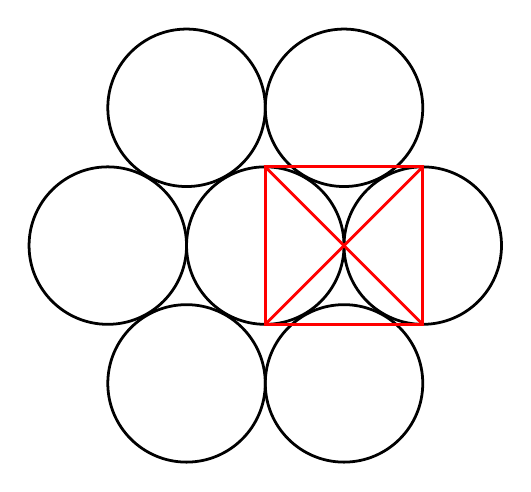
\begin{tikzpicture}
    % ---------------------------------------------
    \draw[line width=1pt] (0, 0) circle[radius=1];
    \draw[line width=1pt] (2, 0) circle[radius=1];
    \draw[line width=1pt] (1, 1.75) circle[radius=1];
    \draw[line width=1pt] (3, 1.75) circle[radius=1];
    \draw[line width=1pt] (-1, 1.75) circle[radius=1];
    \draw[line width=1pt] (0, 3.5) circle[radius=1];
    \draw[line width=1pt] (2, 3.5) circle[radius=1];
    \draw[line width=1pt, color=red] (1, 0.75) rectangle(3, 2.75);
    \draw[line width=1pt, color=red] (1, 0.75) -- (3, 2.75);
    \draw[line width=1pt, color=red] (3, 0.75) -- (1, 2.75);
  \end{tikzpicture}
  \caption{Particles bonded to neighbours}
  \label{fig:bonded_dem}
\end{figure}

As a first step in simulating an elastic body using bonded DEM is to discretize
the body into particles having finite radius and mass, connected to its
neighbours with relaxed springs in tangential and normal directions. The
dynamics of the body is investigated in terms of each particle rather than
looking at the full body collectively. The forces on each particle due to its
neighbours are governed by Hertz model. The forces from external sources other
than the particles of the body are can also be easily integrated into the forces
of the particle using Hertz law.


The accuracy of the results depend on the efficiency of the packing of solid.  A
coordination number around six will give approximation and the structure will be
stable. To get a optimum packing one needs to follow specific packing mechanisms
rather than using a structured grid.


\section{Coupling Bonded DEM with SPH}
\label{sec:coupling-bonded-dem}


\citeauthor{wu-2016-coupl-sph} coupled SPH with bonded DEM to simulated
deformation of elastic structures under fluid flow. Till now, we modelled fluid
using SPH, rigid and elastic solids by DEM and bonded DEM\,. The interaction of
a fluid particle with solid can be modelled using boundary-fluid pressure force.

Force between any two particles can be directly derived from SPH principles
as
\begin{equation}
  F^p_{i \leftarrow j} = -m_{i} m_{j} \frac{p_{i}}{\rho^2_{i}}
\end{equation}
From this, force exerted by a fluid particle on a solid particle is can be
derived as
\begin{equation}
  F^p_{f_i \leftarrow b_j} = -m_{f_i} \psi_{b_j}(\rho o_{i}) \frac{p_{f_i}}{\rho^2_{f_i}}
\end{equation}
Where $\psi_{b_j}(\rho o_{i}) $ is $\rho_o \, V_{b_j}$. While computing the
force between the fluid and solid particle, solid particle is assigned with
volume. In the force equation rather than using the mass of the solid particle
we should use the volume of the solid and the density of the fluid. An equal and
opposite force is applied by boundary particle on the fluid

\begin{equation}
  F^p_{b_i \leftarrow f_j} = -F^p_{f_i \leftarrow b_j}
\end{equation}


%%

%%% Local Variables:
%%% mode: latex
%%% TeX-master: "../mainrep"
%%% End:

%  LocalWords:  Baraff

% 
\chapter{Literature Survey}

The bibliographic entries are to be kept in a file named
\verb|<something>.bib|. In this sample report we call it as
\verb|mylit.bib|. This file must be included without the \verb|.bib|
extension in the main file as: \verb|\bibliography{mylit}|.   Open the
file \verb|mylit.bib| to see the format in which the entries are
written. This is written in the Bib\TeX format. Most of the
bibliographic web pages (Scopus, ISI Web) and software (EndNote, etc)
allow you to export bibliographic entries in the Bib\TeX format.

Citations are referred in the text using \verb|\citet| command which produces citations as though they are part of the text.  In order to say
somebody did this work as a part of a line use:
\verb|\citet{Batzri1973}| have done extensive work on \ldots.  This will produce
\citet{Batzri1973} have done extensive work on \ldots. Alternately citations can appear in parenthesis.  
The command~\verb|\citep{Batzri1973}| is used to automatically put the
citations in parenthesis.  As an example consider the extensive work
done in the area of book writing \citep{Sackmann1995a,Boal2012}.

Conferences \citep{rich-mart92} or collection of work
\citep{Sackmann1995a} also have special entries.

It is also possible to cite thesis like this:
\citet{jariwala00,luding94} or just unpublished work from
\citet{SunHI03}. Some times there are unclassified bibliographic
entries which can be put under ``misc'' \citep{Smith99}.



%%% Local Variables: 
%%% mode: latex
%%% TeX-master: "../mainrep"
%%% End: 

% 
\chapter{Literature Survey}

The bibliographic entries are to be kept in a file named
\verb|<something>.bib|. In this sample report we call it as
\verb|mylit.bib|. This file must be included without the \verb|.bib|
extension in the main file as: \verb|\bibliography{mylit}|.   Open the
file \verb|mylit.bib| to see the format in which the entries are
written. This is written in the Bib\TeX format. Most of the
bibliographic web pages (Scopus, ISI Web) and software (EndNote, etc)
allow you to export bibliographic entries in the Bib\TeX format.

Citations are referred in the text using \verb|\citet| command which produces citations as though they are part of the text.  In order to say
somebody did this work as a part of a line use:
\verb|\citet{Batzri1973}| have done extensive work on \ldots.  This will produce
\citet{Batzri1973} have done extensive work on \ldots. Alternately citations can appear in parenthesis.  
The command~\verb|\citep{Batzri1973}| is used to automatically put the
citations in parenthesis.  As an example consider the extensive work
done in the area of book writing \citep{Sackmann1995a,Boal2012}.

Conferences \citep{rich-mart92} or collection of work
\citep{Sackmann1995a} also have special entries.

It is also possible to cite thesis like this:
\citet{jariwala00,luding94} or just unpublished work from
\citet{SunHI03}. Some times there are unclassified bibliographic
entries which can be put under ``misc'' \citep{Smith99}.



%%% Local Variables: 
%%% mode: latex
%%% TeX-master: "../mainrep"
%%% End: 

% 
\chapter{Materials and Methods}

\section{Including Figures}

Figures are conveniently included using postscript format.  If you are
generating a figure in a software, please check if the software
supports writing to a postscript or a PDF format. This format is loss
less vector format and with reproduce in any magnification without any
pixelation. Make sure to write it to an ``Encapsulated Post-script''or
.eps format.


\begin{figure}[tbp]
  \centering
    \includegraphics[width=0.7\textwidth]{profflow}
    \caption[Process flow sheet]{Process flow sheet of the
      experimental setup. The caption of the figure goes here. A
      shorter caption can be written in square brackets to identify it
      in the list of figures.}
    \label{fig:pfs} 
\end{figure}

Figures should be given a label and which can be used to refer to them
in the running text using \verb|\ref{}| command. Figure~\ref{fig:pfs}
describes the process flow sheet of the experimental set up used in
this report. The \Figref{fig:pfs} can also be refered by a short form notation
a pre-defined macro \verb"\Figref".



%%% Local Variables: 
%%% mode: latex
%%% TeX-master: "../mainrep"
%%% End: 

% \chapter{Results and Discussions}


\section{Including Tables}

Tables are to be used in a special environment so that they have a
Number, caption and appear in the list of tables.
Table~\ref{tab:samtab} is a sample table. In the case of tables, it is
a convention to write the caption above the table.  Note that in the
case of figures the caption appears below the figure.

\begin{table}[tbp]
  \centering
    \caption{Physical properties of the materials used.}
    \label{tab:samtab}
    \begin{tabular}{ll}
      \toprule 
      Property & Value \\
      \midrule
      Particle Density, $\rho_{\mathrm{p}}$ & 2500 kg/m$^{3}$ \\
      Viscosity, $\eta_{\mathrm{s}}$& 1 $\times 10^{-3}$ Pa-s \\
      \bottomrule \\
    \end{tabular}  
\end{table}

%%% Local Variables: 
%%% mode: latex
%%% TeX-master: "../mainrep"
%%% End: 


%****************************************************************
%                         Appendices
%****************************************************************
%% Additional, supporting material, such as codes, derivations, etc., can be placed in the appendix
\appendix
\chapter{Supporting Material}

%******************************************************************
%                         Bibliography or References
%******************************************************************
\bibliography{mylit}

%*******************************************************************
%                         List of publications
%******************************************************************
%%%
\listofpublications


\noindent Put your publications from the thesis here. The packages \texttt{multibib} or \texttt{bibtopic} or \texttt{biblatex} or enumerate environment or thebibliography environment etc. can be used to handle multiple different bibliographies in the document.








%%======================================================================
%%% Local Variables: 
%%% mode: latex
%%% TeX-master: "../mainrep"
%%% End: 









%*******************************************************************
%                        Acknowledgements
%*******************************************************************
%%%
\acknowledgments

This section is for the acknowledgments. Please keep this brief and resist the temptation of writing flowery prose! Do include all those who helped you, e.g. other faculty/staff you consulted, colleagues who assisted etc.






\signature{\today}
%\signature[Indian Institute of Technology Bombay]{\today}

%========================================================================

%%% Local Variables: 
%%% mode: latex
%%% TeX-master: "../mainrep"
%%% End: 


%*******************************************************************
%                        About author
%*******************************************************************
\colophon % remove this command while using this file.

% GAME OVER
%*******************************************************************
\end{document}

%%% Local Variables:
%%% mode: latex
%%% TeX-master: t
%%% End:
